\chapterstart{第二阶段：原理发现}
\label{sec:principles}

第一阶段已经证明，改变文本组织和学习方式可以改善模型。第二阶段把这些实践结果转化为科学问题，围绕经验与表示、学习目标、结构与能力复用、学习动力学和测量方法开展研究。Qiushi Engine 从观察中提出解释，构造能够区分解释的对照，实施实验并根据结果调整认识。研究既形成可指导下一代模型的训练原则，也形成具有独立价值的理论构造、机制分析和实验方法。

本章展开其中两条相互补充的证据链：不同训练经验怎样改变模型利用上下文的方式，以及所学能力能否被新输入使用、能否经受后续训练。前一部分主要使用自然文本，后一部分使用能够精确改变关系和内部计算的受控任务。两类实验共同为下一阶段的训练设计提供依据。其他研究分支按其科学问题在第\ref{sec:lineage}章展开，具体方法、实验和结论状态保留在附录\ref{app:catalog}与配套研究材料中。

\subsection{关系类型塑造上下文使用方式}
\label{sec:relation}

逐字重复提供相同表达的再次呈现，对齐重述则把相关内容放入不同表达。两种安排都增加相关文本的接触，但对模型的预测要求不同。若它们只是可互换的信息曝光，则在相近预算下应产生近似的来源利用行为；如果模型练习的是特定的来源—目标关系，收益应依赖后续目标与训练关系是否一致。

例如，来源叙述某个物体的位置，后文用不同句式再次描述该位置。预测后文被遮盖的地点时，模型既可能读取前文，也可能只依据附近词语的常见搭配。若把真实来源换成等长无关文本，目标不变，预测差异就能测量这段来源带来的作用。来源—重述关系因而提供了一类具体的上下文依赖，用于比较训练经验怎样影响后续预测。

各条件共同继承已有改写语料。在此基础上，参照条件不增加所研究的紧凑配对，另外两组分别增加逐字重复和对齐重述，用来比较新增经验的关系类型。研究再为两类配对分别构造同窗与分窗条件：同窗时，来源与对应文本进入同一次预测的上下文；分窗时，保留各自全部材料，但放入不同窗口，使一次预测无法同时访问两者。这样，关系类型的比较与保持文本不变的窗口比较各自对应明确变量。

为直接测量来源的作用，研究保持待预测的词不变，分别提供真实来源、无关来源和长度匹配的普通中性文本。若模型给正确词的概率为 $p$，负对数似然（negative log-likelihood，NLL）就是 $-\log p$；概率越高，NLL 越低，表示预测越好。使用自然对数时单位为 nat。对多个确定的正确目标取平均，得到这里使用的交叉熵损失（cross-entropy，CE）。记三种输入条件下的平均损失为 $T,U,N$，定义
\begin{equation}
 A_T=N-T,\qquad A_U=N-U.
\label{eq:source_advantage}
\end{equation}
$A_T$ 越大，表示真实来源相对中性文本越有帮助。$A_U$ 则检查无关来源是否也产生类似变化。两者分别称为真实来源优势和无关来源优势，用来测量指定目标上的上下文作用。例如，真实来源明显改善预测、无关来源变化较小，就支持相关内容本身发挥了作用。

评测进一步按目标 token 是否出现在来源中分组。具体比较的是分词器给出的编号：编号相同即归为重合，否则归为不重合。这种分类测量词面片段的重复，不直接判定完整单词、事实或语义是否新颖。图\ref{fig:relation}采用紧凑重述中 token 不重合的目标。

\begin{figure}[htbp]
\centering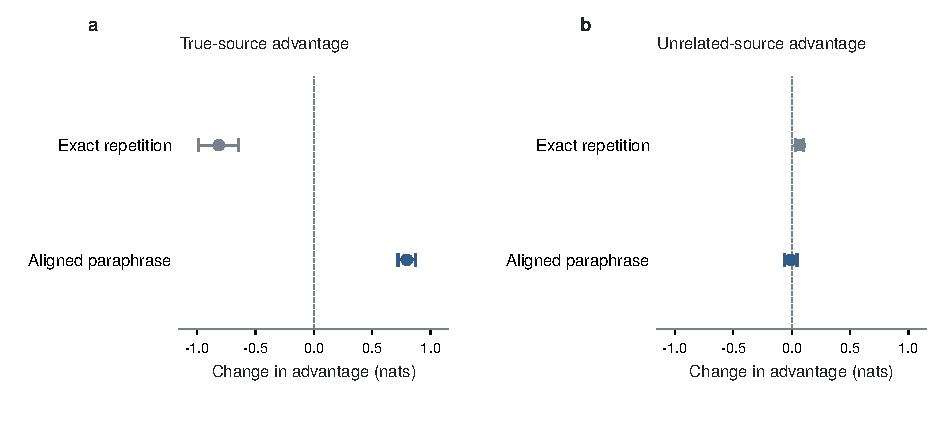
\includegraphics[width=\linewidth]{figures/relation_context_use.pdf}
\caption{训练关系对来源信息利用的影响。a，真实来源优势；b，无关来源优势。横轴为相对参照模型的优势变化，单位为 nats，优势定义见式\eqref{eq:source_advantage}。评测目标为紧凑重述中未在来源出现的 token。点表示三个训练种子的均值，误差线表示种子间标准差。}
\label{fig:relation}
\end{figure}

三个训练种子中，相对参照，逐字重复使该目标类别的真实来源优势平均变化 $-0.8138$ nats，对齐重述为 $+0.7970$ nats；种子标准差分别为 0.1729 与 0.0758（图\ref{fig:relation}）。两种经验产生相反方向的效果，而无关来源优势只分别变化约 $+0.0679$ 与 $-0.0085$ nats。

这一差异究竟来自材料本身，还是来自模型如何共同使用这些材料？表\ref{tab:relation_windows}给出两个种子的窗口对照。对逐字重复和对齐重述分别保留原材料，只把关系两端分开，原来较大的负效应与正效应都明显减弱。文本仍在训练中出现，但不再作为同一次预测的上下文共同发挥作用。这说明，组织有限经验不仅要决定放入哪些文本，还要决定一次预测能利用它们之间的什么关系。

\begin{table}[htbp]
\caption{保持各自配对材料的窗口对照。数值为相对参照的真实来源优势变化 $\Delta A_T$（nats），采用 80M、90M、100M 词检查点的均值；每个检查点测量 2,732 个来源不重合目标，两列对应不同训练种子。}
\label{tab:relation_windows}
\small
\begin{tabularx}{\linewidth}{@{}Ylrr@{}}
\toprule 训练关系 & 窗口组织 & 种子 43022 & 种子 43122\\\midrule
\input{tables/relation_windows}
\end{tabularx}
\end{table}

英文维基百科与 Simple English 的自然重述材料进一步揭示了目标依赖性。表\ref{tab:natural_restatement}使用 1,200 个来源对，分别比较目标 token 在来源中出现与未出现两类情况。对齐重述在句式改变、目标片段仍见于来源的条件下，提高了真实来源的预测帮助；目标 token 不在来源中时，其优势接近参照，而逐字重复产生负效应。这里，训练经验并未带来不加区分的迁移：不同表达中的内容复用与来源外目标预测，对模型提出了不同要求。

\begin{table}[htbp]
\caption{自然重述文本上的关系迁移。数值为相对参照的 $\Delta A_T$（nats），先在每个来源对的同类目标内平均，再对来源对平均；报告三个训练种子的均值与标准差。每种目标类别均包含 1,200 个来源对，类别按 token 编号是否见于来源划分。}
\label{tab:natural_restatement}
\small
\begin{tabularx}{\linewidth}{@{}Yrr@{}}
\toprule 预测目标 & 逐字重复 & 对齐重述\\\midrule
\input{tables/natural_restatement}
\end{tabularx}
\end{table}

因此，有限经验的价值具有关系选择性：训练中练习的关系与测试所需关系是否相符，会改变迁移的方向。同窗—分窗比较说明关系何时能够参与学习，自然重述比较则说明这种学习能帮助哪些目标。这两组结果共同把“更多相关文本”细化为可以检验的经验组织原则。

这组结果与相关文献构成直接联系。相关文档组织、训练分布与上下文学习之间已有研究\citep{shi2024incontext,chan2022distribution,haga2024variationsets}。Chen 等通过删除预训练文本中的平行结构，直接研究了同窗关系对上下文学习的影响\citep{chen2024parallel}；重复也可以促进某些注意力机制的形成\citep{zucchet2025sparse}。本文进一步辨明具体关系与目标之间的对应条件：逐字重复和重述在哪些目标上产生不同方向的效果，各自保持文本而拆分窗口后发生什么，以及哪些迁移没有出现同样收益。

\subsection{熟悉表现与新输入上的能力复用}
\label{sec:reach}

模型学会处理一种关系后，新的名字或符号能否使用同样的能力？这要求把熟悉题目的表现与新对象上的关系处理分开测量。本文用“调用范围”描述同一种已学计算能够被哪些输入使用。例如，模型能按熟悉名字选出正确属性，换成新名字后能否继续完成同一操作？研究采用四选一关系任务，分别测量熟悉符号与未见符号，并直接干预与答案选择有关的内部信号。

任务先给出查询对象，再给出四个对象与属性的对应，要求返回被查询对象的属性。可以用“查询 B；A 对应红色，B 对应蓝色，C 对应绿色，D 对应黄色”理解其结构，正确答案为蓝色；这里的词语仅用于解释，实际实验使用受控符号。测试中可以保持关系规则，换成未参与相应关系训练的查询符号，也可以在包含未见对象的上下文中继续查询熟悉对象。后一个比较帮助区分“上下文含有陌生符号”与“模型不能用陌生查询选择正确属性”。

比较中的全序列监督使用序列预测目标，关系答案监督则强调查询答案位置上的预测。静态权重方案固定两类学习信号的相对权重；交替方案轮换关系答案与全序列监督。图\ref{fig:reach}报告用于功能干预分析的两个训练种子（43、100）的均值；这两个种子在初始关系学习后均已表现出未见符号迁移。初始关系学习后，熟悉准确率为 100.0\%，未见准确率为 87.5\%。普通全序列续训后，熟悉准确率为 87.2\%，未见准确率降至 40.2\%。静态关系权重条件的未见准确率为 75.5\%，交替监督为 83.3\%，两者的熟悉准确率均为 100.0\%。监督分配因而改变了新符号使用已学关系的能力。

\begin{figure}[htbp]
\centering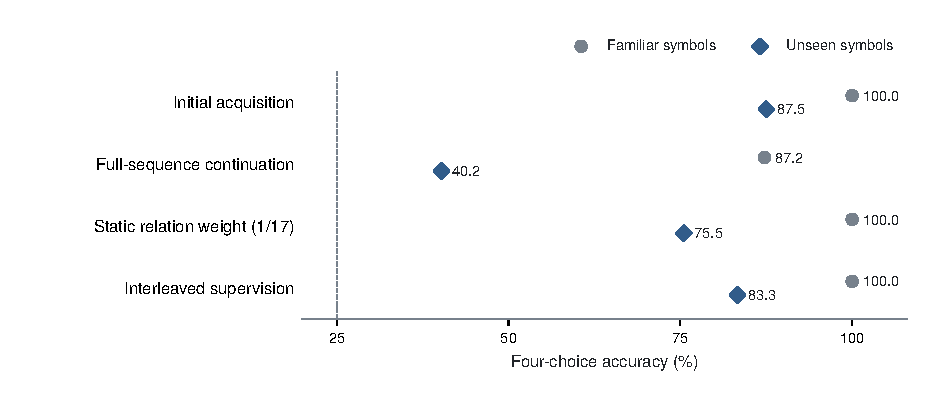
\includegraphics[width=\linewidth]{figures/interface_reach.pdf}
\caption{受控关系任务中熟悉符号与未见符号的四选一准确率。比较初始学习、全序列续训、静态关系监督与交替监督四种设置。点为两个训练种子的均值，虚线表示 25\% 机会水平。静态关系监督权重为 $1/17$；交替监督轮换关系答案目标与全序列目标。}
\label{fig:reach}
\end{figure}

仅比较准确率，还不能知道哪一种内部计算参与了回答。模型在每个属性位置都有一个内部数值表示，称为隐藏状态。研究在第一层比较被查询位置与其他位置的平均隐藏状态，将二者的差归一化，得到一个与位置选择相关的方向。该方向由初始关系模型的 1,000 个拟合样本确定，随后固定用于各续训条件；各类测试分别使用 384 个样本。干预只修改这个方向上的数值，其余分量不变：中心化把四个位置的投影值设为相同，置零删除这一分量，旋转则把这组数值在四个位置间循环搬移。若删除后答案变差、搬移后答案跟随移动，就能检验这个信号是否实际影响了选择。

初始模型的未见准确率从 87.5\% 降至置零后的 25.0\%；交替监督条件从 83.3\% 降至 38.7\%。这些变化说明，被干预的信号对相应任务具有功能作用。旋转之后的目标选择率检验回答是否指向新位置，不应与原题准确率混淆。

\begin{table}[htbp]
\caption{未见符号上的内部功能干预。前三个数值列为原题准确率；最后一列为旋转内部信号后，答案跟随信号指向新位置的比例。所有数值单位为\%，采用图\ref{fig:reach}的同一实验设置。}
\label{tab:intervention}
\begin{tabularx}{\linewidth}{@{}Yrrrr@{}}
\toprule 条件 & 原始 & 中心化 & 置零 & 干预目标选择率\\\midrule
初始获得 & 87.5 & 26.6 & 25.0 & 67.6\\
普通全序列续训 & 40.2 & 25.1 & 31.1 & 31.4\\
静态关系监督权重 & 75.5 & 31.3 & 33.6 & 48.2\\
交替关系监督 & 83.3 & 32.9 & 38.7 & 63.9\\
\bottomrule
\end{tabularx}
\end{table}

连续训练中的测量进一步区分了能力下降与后续恢复：普通全序列续训先削弱了答案选择信号，随后恢复了熟悉查询对这一信号的使用，但未见查询没有同步恢复。查询熟悉对象时，即使上下文包含未见对象，模型仍可正确使用该信号。这将问题定位到哪些查询能够调用已学计算，而非对陌生上下文的普遍不适应。

研究还检验了一种替代解释：普通续训后，相关信息是否转移到了另一条线性方向？为此，分别从熟悉查询、单个未见查询和两个未见查询的隐藏状态中重新拟合方向，将拟合样本与测试样本分开，再沿新方向替换答案选择信号，以回答转向指定位置的比例衡量干预效果。重新拟合的方向在这里用作干预工具，所测的是它能否控制模型的选择。普通全序列续训模型在这些方向上的未见查询重定向仍弱于交替监督模型，因而没有支持“换一个线性方向即可找回同样功能”的解释。此类内部干预将表示中可读出的信息与实际参与回答的计算联系起来\citep{geiger2021causal,zhang2024patching}。

上下文学习在训练中的消退，以及熟悉与未见 token 上采用不同策略，已有相关研究\citep{singh2023transient,anand2025dual}。Dual Process Learning 通过权重遗忘研究这两种策略的共存。本研究进一步改变关系监督的分配，并用删除、搬移内部信号的实验检查其功能。新增结果具体落在监督条件如何影响复用，以及哪些内部信号仍能被新符号使用。

\subsection{监督分配如何改变关系学习}

来源文本出现于输入，只是关系学习的一个前提。如果重述附近的词已经足以补全目标，模型可以降低损失，却很少需要读取来源。监督分配进一步决定哪些预测受到训练、各类预测占多大权重。删除局部线索、改变目标位置或调整损失权重，都是改变这种分配的操作；研究需要同时测量关系能力与其他语言功能。

受控实验通过普通全序列监督、关系答案监督、交替安排及匹配有效权重，区分关系学习与其他预测任务之间的资源分配。关系不匹配的答案监督及单纯降低上下文压力，不能复现全部目标行为。因而，结果并不只是“减小总损失”或“增加关系文本”所能概括；监督位置与被监督的关系是否对应，是必要的实验变量。

紧凑重述的目标删除实验从另一个方向检验监督内容。来源外目标指目标词没有出现在配对的来源段落中；复制目标指在来源中能够逐词匹配的目标。研究保留全部输入文本，分别删除这两类目标中的一部分预测损失。累计 100M 词后，完整监督条件的七项均值为 43.896，删除来源外目标为 43.437，删除匹配复制目标为 42.792。相同输入下，参与监督的目标集合改变了后续表现。两种删除条件移除的目标数量接近而非完全相同，完整条件又有更多监督目标，因此该比较同时涉及监督内容和数量。

另在累计曝光 20M 词的目标删除模型上，研究测量了不与相应训练来源对重合的局部预测。在 710 个来源对、974 次目标预测上，删除来源外监督相对删除匹配复制目标，使被测来源外目标的损失高出 0.0796 nats。按来源对重新抽样，95\% 区间为 $[0.031,0.125]$；进一步要求整个来源文档独立后，区间包含零，尚不能确认同样差异。这里的早期局部预测与前述 100M 词后的七项评价回答不同问题：删去哪类目标会损伤指定内容的预测，以及不同监督安排如何影响晚期综合表现。附录\ref{app:extended}分别给出结果。

这些结果说明，应分别检查输入是否提供所需关系、预测目标是否要求使用该关系，以及分配给这些目标的学习信号是否足够。输入遮盖与预测比例的分离已有直接研究\citep{wettig2023mask}；本研究把这一设计用于来源—重述关系，检验同样文本怎样因监督位置不同而产生不同学习结果。

\subsection{经验的价值依赖预算、替代对象与能力状态}

同一种数据是否有价值，不能脱离它替代了什么。给模型增加一种经验，同时删去等量另一种经验，所估计的是一个替换效果。设 $A$ 是加入的经验，$D$ 是被移除的经验，$B$ 为参照训练流，则在固定训练配置下可以定义
\begin{equation}
 \Delta_T(A,D;B)=Y_T(B-D+A)-Y_T(B).
\label{eq:substitution}
\end{equation}
其中 $Y_T$ 表示在训练进度 $T$ 的评价结果，$B-D+A$ 表示从原训练材料中移除 $D$、加入 $A$。比较固定预算、架构、训练日程和随机种子。这个定义将新增数据与被替代数据的作用放在同一比较中，使“数据是否有价值”成为针对明确参照的实验问题。

研究中的晚期 DeBERTa 比较显示，视图改造、经验覆盖扩展与精确重复相对各自参照呈现不同效果；在另一 RoBERTa 配置中，视图方案虽然改善了自身训练目标，却没有产生相同的广泛指标收益。文本来源也不是可互换的资源：固定加入内容后，移除儿童导向语料还是成人文字，会改变最终结果。由此应保留的是条件化的认识：经验价值取决于被替代的信息、学习阶段和模型状态，不能从一个早期损失或一个文本分布距离推导普遍排序。

这组研究还辨明了结构比较中的初始化混淆。随机种子确定伪随机数序列；新增网络层会改变这串数被各参数使用的次序，因此相同种子未必使共同参数得到相同初值。研究显式复制共同参数后，原先较大的负交互明显减弱。这里的交互指同一种数据处理在不同模型结构上带来的收益差异。该结果说明，控制共同参数的实际初值，是判断结构与数据如何共同作用的重要条件。

\subsection{可操作原则与独立成果}

第二阶段将有限经验学习的设计问题落实为三个可分别操纵的条件：预测时哪些信息可见，哪些目标及其权重参与学习，以及后续训练中哪些已有功能需要保持。自然文本对照揭示关系与窗口的作用，受控任务揭示能力对新输入的可用范围，两类证据共同指向输入、监督与保持的协同设计。

这些认识改变了下一阶段要作出的设计选择：固定监督目标、扩大局部遮盖，观察模型是否改变对来源的使用；固定遮盖、增加预测目标，检查收益是否来自监督数量；改变保持约束所用的输入，检查新学习与已有功能怎样变化。Qiushi Engine 将原本围绕高分配置的探索，推进为对信息可见性、监督分配和功能保持的分别设计与检验。第三阶段把这些问题落实到真实模型训练，并用对照结果继续修正判断。

研究还形成了关系锚点、共享表示空间、身份匹配、实体存储与测量设计等独立成果。第\ref{sec:lineage}章说明它们各自研究什么、已验证到哪里，附录\ref{app:catalog}提供主题目录。主线进入第三阶段时保留的是可以转化为输入、监督与保持操作的认识；其他有效成果按自身问题保存，不以是否进入最终模型决定其价值。
